% What most papers load. The text uses each package, so its fonts and lazily
% loaded files are cached too.
\documentclass{article}
\usepackage[utf8]{inputenc}
\usepackage[T1]{fontenc}
\usepackage[margin=1in]{geometry}
\usepackage{amsmath,amssymb,amsthm,mathtools,bm}
\usepackage{graphicx,xcolor,booktabs,array,caption,subcaption,enumitem,microtype}
\usepackage{listings}
\usepackage{siunitx}
\usepackage{tikz}
\usetikzlibrary{arrows.meta,calc,positioning,shapes.geometric,fit,backgrounds}
\usepackage{hyperref}
\usepackage{cleveref}
\newtheorem{theorem}{Theorem}
\lstset{language=Python,basicstyle=\ttfamily\small,frame=single,numbers=left}
\begin{document}
\tableofcontents
\section{Text}\label{sec:text}
\textbf{Bold} \textit{italic} \emph{\textbf{both}} \texttt{code} \textsf{sans}
\textsc{Small Caps} {\tiny a}{\footnotesize a}{\small a}{\large a}{\Large a}{\Huge a}
See \cref{sec:text}, \url{https://example.com}, and \href{https://example.com}{this}.\footnote{Note.}
\begin{itemize}[nosep]\item One\end{itemize}
\begin{theorem}Proved. \qed\end{theorem}
\section{Math}
\begin{equation}\label{eq}
\int_0^\infty \sum_{i=1}^n \bm{x}_i\,\mathbb{R}\mathcal{L}\mathfrak{g}\mathrm{d}x \leq \sqrt{\frac{a}{b}} \mathbf{v}
\end{equation}
$x^{y^z} \in \mathbb{R}$ and {\small $x^{y^z}$} and {\large $x^{y^z}$}
\section{Units and code}
\SI{9.81}{\metre\per\second\squared}, \qty{20}{\celsius}, \num{1.2e-3}, \ang{30}
\begin{lstlisting}
def f(x):  # comment
    return "string"
\end{lstlisting}
\begin{table}[h]\centering
\begin{tabular}{lS[table-format=2.1]}\toprule A & {B} \\\midrule a & 10.5 \\\bottomrule\end{tabular}
\caption{Table}\end{table}
\begin{figure}[h]\centering
\begin{subfigure}{.4\textwidth}
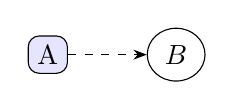
\begin{tikzpicture}
\node[draw,rounded corners,fill=blue!10] (a) {A};
\node[draw,ellipse,right=of a] (b) {$B$};
\draw[-{Stealth},dashed] (a) -- ($(a)!.5!(b)$) -- (b);
\end{tikzpicture}\caption{Part}\end{subfigure}
\caption{Figure}\end{figure}
\end{document}
